% Macro momentum, out of sample. Build: latexmk -xelatex macro_momentum.tex
% Audience: a college freshman with basic finance and macro. Every term is
% explained the first time it appears; the glossary is the last slide.
% Numbers, tables and figures come from scripts/make_deck_assets.py; do not
% type results into this file, use the \n... macros in generated/numbers.tex.
\documentclass[aspectratio=169,10pt]{beamer}
\usetheme[progressbar=frametitle,numbering=fraction,sectionpage=progressbar]{metropolis}

\usepackage{fontspec}
\setsansfont{FiraSans}[Extension=.otf, UprightFont=*-Light, BoldFont=*-Medium,
  ItalicFont=*-LightItalic, BoldItalicFont=*-MediumItalic]
\setmonofont{FiraMono}[Extension=.otf, UprightFont=*-Regular, BoldFont=*-Medium]
\usepackage{booktabs,tabularx,array,graphicx}
\usepackage{tikz}
\usetikzlibrary{positioning,arrows.meta,calc}
\usepackage{appendixnumberbeamer}
\tikzset{cbox/.style={draw=#1,line width=0.8pt,rounded corners=2pt,fill=white,
  minimum width=2.6cm,minimum height=0.8cm,align=center,font=\small}}

% generated by scripts/make_deck_assets.py, do not edit
\newcommand{\nMMRet}{7.3\%}
\newcommand{\nMMVol}{10.7\%}
\newcommand{\nMMSharpe}{0.69}
\newcommand{\nMMT}{2.2}
\newcommand{\nMMDD}{$-$15.4\%}
\newcommand{\nMMNetRet}{6.0\%}
\newcommand{\nMMNetSharpe}{0.57}
\newcommand{\nMMTurn}{40}
\newcommand{\nMMDrag}{1.3\%}
\newcommand{\nMMSharpeTwo}{0.44}
\newcommand{\nMMSharpeFour}{0.20}
\newcommand{\nMMFirstHalf}{0.25}
\newcommand{\nMMSecondHalf}{1.19}
\newcommand{\nTFRet}{$-$0.6\%}
\newcommand{\nTFVol}{10.7\%}
\newcommand{\nTFSharpe}{$-$0.05}
\newcommand{\nTFT}{$-$0.2}
\newcommand{\nTFDD}{$-$22.8\%}
\newcommand{\nTFNetRet}{$-$1.4\%}
\newcommand{\nTFNetSharpe}{$-$0.13}
\newcommand{\nTFTurn}{24}
\newcommand{\nTFDrag}{0.8\%}
\newcommand{\nTFSharpeTwo}{$-$0.20}
\newcommand{\nTFSharpeFour}{$-$0.34}
\newcommand{\nTFFirstHalf}{$-$0.02}
\newcommand{\nTFSecondHalf}{$-$0.10}
\newcommand{\nMixRet}{3.4\%}
\newcommand{\nMixVol}{8.7\%}
\newcommand{\nMixSharpe}{0.39}
\newcommand{\nMixT}{1.2}
\newcommand{\nMixDD}{$-$9.5\%}
\newcommand{\nMixNetRet}{2.5\%}
\newcommand{\nMixNetSharpe}{0.29}
\newcommand{\nMixTurn}{26}
\newcommand{\nMixDrag}{0.8\%}
\newcommand{\nMixSharpeTwo}{0.20}
\newcommand{\nMixSharpeFour}{0.00}
\newcommand{\nMixFirstHalf}{0.15}
\newcommand{\nMixSecondHalf}{0.63}
\newcommand{\nMMBondTurn}{22}
\newcommand{\nMMFxTurn}{11}
\newcommand{\nMMEqTurn}{8}
\newcommand{\nCorrMMTF}{0.31}
\newcommand{\nCorrMMEq}{$-$0.27}
\newcommand{\nCorrMMBond}{$-$0.08}
\newcommand{\nStart}{Nov 2016}
\newcommand{\nEnd}{Oct 2026}
\newcommand{\nMonths}{120}
\newcommand{\nSharpeSE}{0.35}
\newcommand{\nCostEq}{4}
\newcommand{\nCostBond}{3}
\newcommand{\nCostFx}{3}
\newcommand{\nMMBondSharpe}{0.82}
\newcommand{\nMMFxSharpe}{0.37}
\newcommand{\nMMEqSharpe}{0.17}
\newcommand{\nMMCycleSharpe}{0.52}
\newcommand{\nMMTradeSharpe}{0.25}
\newcommand{\nMMMonetarySharpe}{0.35}
\newcommand{\nMMRiskSharpe}{0.67}
\newcommand{\nMMXSSharpe}{0.94}
\newcommand{\nMMTSSharpe}{0.23}
\newcommand{\nMMLagZero}{0.69}
\newcommand{\nMMLagZeroNet}{0.57}
\newcommand{\nMMLagOne}{0.65}
\newcommand{\nMMLagOneNet}{0.52}
\newcommand{\nMMLagTwo}{0.21}
\newcommand{\nMMLagTwoNet}{0.09}


% Series colours match the figures (reference categorical slots 1-3).
\definecolor{mmblue}{HTML}{2A78D6}
\definecolor{tforange}{HTML}{EB6834}
\definecolor{mixaqua}{HTML}{1BAF7A}
\definecolor{ink}{HTML}{23373B}
\definecolor{ink2}{HTML}{52514E}
\definecolor{muted}{HTML}{8A8984}
\definecolor{longc}{HTML}{D7E6F8}
\definecolor{shortc}{HTML}{FBDCCF}
\definecolor{boxbg}{HTML}{F3F2EE}
\setbeamercolor{alerted text}{fg=tforange}
\setbeamercolor{block title}{bg=boxbg,fg=ink}
\setbeamercolor{block body}{bg=boxbg!50}

% Source footer: every slide with a number or a claim carries one.
\newcommand{\src}[1]{%
  \begin{tikzpicture}[remember picture,overlay]
    \node[anchor=south west,inner sep=0pt,text width=0.86\paperwidth,align=left,
          font=\fontsize{6}{7}\selectfont,text=muted]
      at ([xshift=0.45cm,yshift=0.22cm]current page.south west) {Source: #1};
  \end{tikzpicture}}
% A short definition box for new terms.
\newcommand{\term}[2]{\colorbox{boxbg}{\parbox{0.95\linewidth}{\footnotesize\textbf{#1}: #2}}\par\vspace{2pt}}
\newcommand{\repo}{\texttt{github.com/chkoh89/macro-momentum}}
\newcommand{\paper}{Brooks (2017), \emph{A Half Century of Macro Momentum}, AQR}

\title{Does macro momentum still work?}
\subtitle{Testing a 2017 investing idea on the ten years that came after it}
\date{\today}
\author{macro-momentum project}
\institute{\repo}

\begin{document}

\maketitle

% ---------------------------------------------------------------------------
\begin{frame}{The question}
  \begin{itemize}
    \item In 2017 a researcher at the investment firm AQR published a strategy called
          \textbf{macro momentum}: buy the markets of countries whose economy has been getting better,
          sell those whose economy has been getting worse.
    \item On data from 1970 to 2016 it looked very good.
    \item But a strategy always looks good on the data it was designed on. The real test is
          what happens \alert{afterwards}.
    \item We rebuilt it with free public data and ran it on \textbf{\nStart{} to \nEnd}, ten years
          the original author never saw.
    \item We also compared it with a simpler, popular strategy: \textbf{trend following}
          (buy what has been going up, sell what has been going down).
  \end{itemize}
  \src{\paper.}
\end{frame}

\begin{frame}{The answer in one slide}
  \begin{columns}[T]
    \begin{column}{0.55\textwidth}
      \begin{itemize}
        \item \textbf{It still worked}, but about half as well as in the original study.
        \item \textbf{Trading costs} eat about a fifth of the profit.
        \item \textbf{Almost all the gains came after 2022}, when inflation and interest rates
              moved a lot.
        \item \textbf{Trend following made nothing} on the same markets over these ten years,
              so a \textbf{50/50 mix} of the two did worse than macro momentum alone.
        \item \textbf{Ten years is not much data}, so treat the exact numbers with caution.
      \end{itemize}
    \end{column}
    \begin{column}{0.41\textwidth}
      \small
      \begin{tabular}{@{}lrr@{}}
        \toprule
        Sharpe ratio & Original & Our test \\
        (higher is better) & 1970--2016 & 2016--2026 \\
        \midrule
        \textcolor{mmblue}{\textbf{Macro momentum}} & 1.2 & \textbf{\nMMSharpe} \\
        \quad after costs & -- & \nMMNetSharpe \\
        \textcolor{tforange}{\textbf{Trend following}} & 1.1 & \nTFSharpe \\
        \textcolor{mixaqua}{\textbf{50/50 mix}} & 1.4 & \nMixSharpe \\
        \bottomrule
      \end{tabular}
      \vspace{0.4em}

      \footnotesize The Sharpe ratio is explained on the next slides. Rough guide:
      0 = no reward for the risk, 0.5 = decent, 1 = excellent.
    \end{column}
  \end{columns}
  \src{\paper; our test: \repo, \texttt{results/summary.md}.}
\end{frame}

% ===========================================================================
\section{The basics in five slides}

\begin{frame}{What can you invest in? Three kinds of market}
  \begin{columns}[T]
    \begin{column}{0.32\textwidth}
      \textbf{Stocks}\\[0.3em]
      \small A \emph{stock index} such as the S\&P 500 (US) or the DAX (Germany) tracks a
      country's biggest companies. It tends to rise when the economy and company profits grow.
    \end{column}
    \begin{column}{0.32\textwidth}
      \textbf{Government bonds}\\[0.3em]
      \small A loan to a government that pays fixed interest. When interest rates in the
      economy \emph{rise}, older bonds paying less become less attractive, so their
      \emph{prices fall}. Bonds dislike inflation and rate hikes.
    \end{column}
    \begin{column}{0.32\textwidth}
      \textbf{Currencies}\\[0.3em]
      \small Holding, say, euros instead of dollars. You gain if the euro strengthens against the
      dollar, and you also earn the interest-rate gap between the two countries.
    \end{column}
  \end{columns}
  \vspace{1em}
  We trade all three in 10 rich countries: US, Germany, Japan, UK, Canada, Australia,
  Switzerland, Sweden, New Zealand, Norway. That is 26 markets in total, because some
  countries have no suitable bond fund.
  \src{\repo, \texttt{src/mm/instruments.py}.}
\end{frame}

\begin{frame}{Long and short}
  \begin{columns}[c]
    \begin{column}{0.55\textwidth}
      \begin{itemize}
        \item \textbf{Going long}: buy something; you profit if its price rises.
        \item \textbf{Going short}: bet on a fall. You borrow and sell it now, buy it back later;
              you profit if the price fell in between.
        \item A \textbf{long-short} portfolio buys the markets it likes \emph{and} shorts the ones it
              dislikes, in equal amounts. If all markets rise or fall together, the two sides cancel.
              It only makes money if its picks beat its pans.
      \end{itemize}
    \end{column}
    \begin{column}{0.42\textwidth}
      \centering
      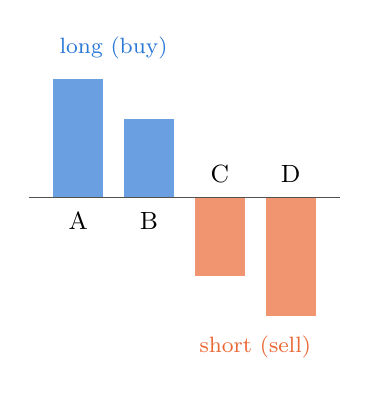
\begin{tikzpicture}[x=0.9cm,y=0.5cm]
        \foreach \c/\h/\col [count=\i] in {A/3/mmblue,B/2/mmblue,C/-2/tforange,D/-3/tforange} {
          \fill[\col!70] (\i-0.35,0) rectangle (\i+0.35,\h);
          \node[font=\small] at (\i,{\h>0 ? -0.6 : 0.6}) {\c};
        }
        \draw[ink2,line width=0.6pt] (0.3,0) -- (4.7,0);
        \node[font=\footnotesize,text=mmblue] at (1.5,3.8) {long (buy)};
        \node[font=\footnotesize,text=tforange] at (3.5,-3.8) {short (sell)};
      \end{tikzpicture}
    \end{column}
  \end{columns}
  \src{Standard definitions; construction in \texttt{src/mm/portfolio.py}.}
\end{frame}

\begin{frame}{Measuring risk and reward}
  \term{Return}{how much the investment gained in a year, in \%. Here always measured
        \emph{above what plain cash in the bank would have earned}, so 0\% means
        ``no better than cash''.}
  \term{Volatility (risk)}{how much the return swings around from month to month. A strategy with
        10\% volatility will, in a typical year, end up within about $\pm$10\% of its average.}
  \term{Sharpe ratio}{return divided by volatility: reward per unit of risk. Lets us compare
        strategies fairly. 0 = no reward, 0.5 = decent, 1 = excellent and rare.}
  \term{Worst fall (drawdown)}{the biggest drop from a previous high, e.g.\ $-15$\% means at one point
        you were 15\% below your best balance so far.}
  \vspace{0.3em}
  \small To compare like with like, every strategy here is scaled to the same risk: about
  \textbf{10\% volatility a year}. A calmer market gets a bigger position, a wilder one a smaller
  position.
  \src{Standard definitions; \texttt{mm.backtest.stats}, \texttt{mm.portfolio.target\_vol}.}
\end{frame}

\begin{frame}{The economy in four numbers}
  \small
  \begin{tabularx}{\textwidth}{@{}l X X@{}}
    \toprule
    Number & What it is & Typical market reaction when it goes \emph{up} \\
    \midrule
    \textbf{GDP growth} & how fast the economy is growing & stocks up, bonds down (rates expected to rise) \\
    \textbf{Inflation} & how fast prices are rising (CPI) & bonds down; stocks down (higher rates ahead) \\
    \textbf{Interest rate} & set (indirectly) by the central bank & bonds down, stocks down, currency up \\
    \textbf{Exchange rate} & value of the currency vs.\ trading partners & exporters hurt, so stocks down \\
    \bottomrule
  \end{tabularx}
  \vspace{0.6em}

  These numbers are published with a delay. GDP for January to March comes out around the end of June.
  A fair test may only use a number \emph{after} it was public.
  \src{\paper, Exhibit 1 and pp.\ 2--3; publication lags in \texttt{src/mm/signals.py}.}
\end{frame}

\begin{frame}{What is a backtest, and why ``out of sample'' matters}
  \begin{itemize}
    \item A \textbf{backtest} asks: if I had followed these rules in the past, what would have happened?
          It is a simulation, not real trading.
    \item The danger: try enough rules on the same history and one will look great by luck.
    \item The cure is an \textbf{out-of-sample test}: freeze the rules, then run them on data the
          designer never saw. That is exactly what we do: the paper's data stop in 2016, ours start there.
    \item We change nothing to make the result look better. All settings come from the paper.
  \end{itemize}
  \vspace{0.5em}
  \centering
  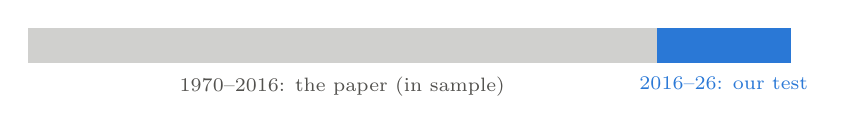
\begin{tikzpicture}[x=0.17cm]
    \fill[muted!40] (0,0) rectangle (47,0.45);
    \fill[mmblue] (47,0) rectangle (57,0.45);
    \node[font=\scriptsize,text=ink2,anchor=north] at (23.5,-0.05) {1970--2016: the paper (in sample)};
    \node[font=\scriptsize,text=mmblue,anchor=north] at (52,-0.05) {2016--26: our test};
  \end{tikzpicture}
  \src{\paper; \repo, \texttt{AGENTS.md} (``Don't tune on the test window'').}
\end{frame}

% ===========================================================================
\section{The strategy}

\begin{frame}{The idea: markets are slow to digest economic news}
  \begin{columns}[c]
    \begin{column}{0.5\textwidth}
      \begin{itemize}
        \item Economies change gradually, and investors take time to adjust prices to the change.
        \item So if a country's economic picture has \textbf{improved over the past year}, its
              markets tend to keep doing well for a while, and vice versa.
        \item Macro momentum (``macro'' = the whole economy) bets on that continuing.
        \item Trend following is its cousin: it uses the \emph{price} itself
              instead of economic data.
      \end{itemize}
    \end{column}
    \begin{column}{0.46\textwidth}
      \centering
      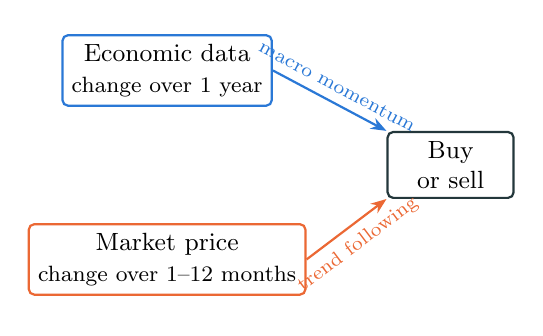
\begin{tikzpicture}[
          arr/.style={-{Stealth[length=2mm]},line width=0.8pt}]
        \node[cbox=mmblue,minimum width=2.4cm] (macro) at (0,1.2) {Economic data\\\footnotesize change over 1 year};
        \node[cbox=tforange,minimum width=2.4cm] (price) at (0,-1.2) {Market price\\\footnotesize change over 1--12 months};
        \node[cbox=ink,minimum width=1.6cm] (pos) at (3.6,0) {Buy\\or sell};
        \draw[arr,mmblue] (macro.east) -- node[midway,above,sloped,font=\scriptsize,text=mmblue] {macro momentum} (pos.north west);
        \draw[arr,tforange] (price.east) -- node[midway,below,sloped,font=\scriptsize,text=tforange] {trend following} (pos.south west);
      \end{tikzpicture}
    \end{column}
  \end{columns}
  \src{\paper, pp.\ 1--3.}
\end{frame}

\begin{frame}{Four themes: what we watch in each country}
  \small
  \begin{tabularx}{\textwidth}{@{}l l X@{}}
    \toprule
    Theme & We look at the change over the past year in\ldots & Example \\
    \midrule
    Business cycle & GDP growth and inflation & growth sped up from 1\% to 3\% \\
    International trade & the currency vs.\ trading partners & the yen lost 10\% \\
    Monetary policy & the short-term interest rate & the central bank raised rates from 1\% to 4\% \\
    Risk sentiment & the stock market's own return & stocks beat cash by 15\% \\
    \bottomrule
  \end{tabularx}
  \vspace{0.6em}

  The original paper used economists' \emph{forecasts} of growth and inflation, which cost money.
  We use the actual published figures instead, used only once they were public.
  \src{\paper, Exhibit 1; data sources in \texttt{docs/data.md}.}
\end{frame}

\begin{frame}{The rule book: what to buy when each number rises}
  \centering
  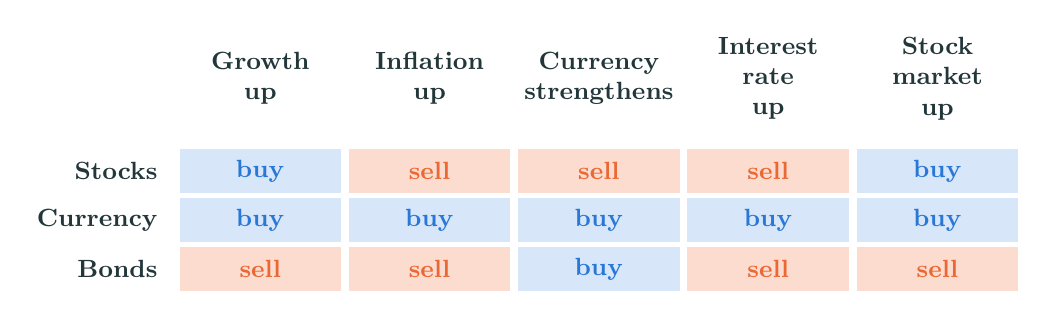
\begin{tikzpicture}[x=2.15cm,y=0.62cm,
      cell/.style={minimum width=2.05cm,minimum height=0.56cm,font=\small,inner sep=0pt},
      hdr/.style={font=\small\bfseries,text=ink,align=center}]
    \foreach \h [count=\i] in {Growth\\up, Inflation\\up, Currency\\strengthens, Interest rate\\up, Stock market\\up}
      \node[hdr,text width=2cm] at (\i,0.9) {\h};
    \foreach \a [count=\j] in {Stocks, Currency, Bonds}
      \node[anchor=east,font=\small\bfseries,text=ink] at (0.45,-\j) {\a};
    \foreach \row [count=\j] in {{1,-1,-1,-1,1},{1,1,1,1,1},{-1,-1,1,-1,-1}}
      \foreach \v [count=\i] in \row {
        \ifnum\v>0
          \node[cell,fill=longc,text=mmblue] at (\i,-\j) {\textbf{buy}};
        \else
          \node[cell,fill=shortc,text=tforange] at (\i,-\j) {\textbf{sell}};
        \fi
      }
  \end{tikzpicture}
  \vspace{0.4em}

  \footnotesize
  \begin{itemize}
    \item \textbf{Bonds} are sold whenever the economy runs hotter or rates rise: both push bond prices down.
    \item \textbf{Currencies} are bought whenever things improve: a strong economy and higher rates attract money.
    \item \textbf{Stocks} are the tricky row: growth helps them, but inflation and rate rises hurt them.
  \end{itemize}
  \src{\paper, Exhibit 1 (written there for a \emph{weaker} currency; same rule, opposite sign); \texttt{src/mm/signals.py}.}
\end{frame}

\begin{frame}{Putting it together}
  \centering
  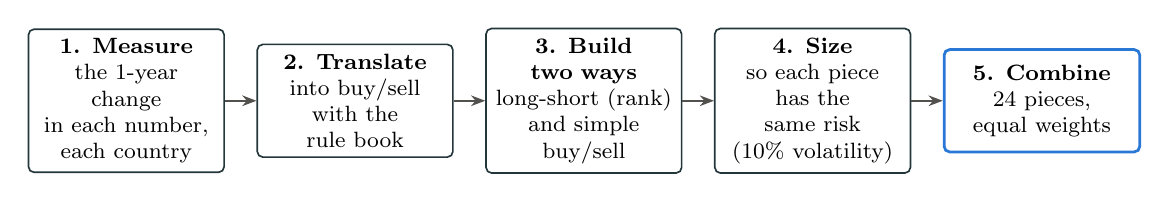
\begin{tikzpicture}[node distance=0.35cm and 0.4cm,
      box/.style={draw=ink,line width=0.6pt,rounded corners=2pt,fill=white,align=center,
                  font=\footnotesize,text width=2.25cm,minimum height=1.3cm},
      arr/.style={-{Stealth[length=1.8mm]},line width=0.7pt,color=ink2}]
    \node[box] (sig) {\textbf{1. Measure}\\the 1-year change\\in each number,\\each country};
    \node[box,right=of sig] (map) {\textbf{2. Translate}\\into buy/sell\\with the rule book};
    \node[box,right=of map] (sty) {\textbf{3. Build two ways}\\long-short (rank)\\and simple buy/sell};
    \node[box,right=of sty] (risk) {\textbf{4. Size}\\so each piece\\has the same risk\\(10\% volatility)};
    \node[box,right=of risk,draw=mmblue,line width=1pt] (agg) {\textbf{5. Combine}\\24 pieces,\\equal weights};
    \foreach \a/\b in {sig/map,map/sty,sty/risk,risk/agg} \draw[arr] (\a) -- (\b);
  \end{tikzpicture}
  \vspace{0.8em}

  \small
  \begin{itemize}
    \item 24 pieces = 3 kinds of market $\times$ 4 themes $\times$ 2 ways of building.
    \item Rebalanced once a month, at the end of the month.
    \item \textbf{Trend following}, for comparison: buy a market if its price rose over the past
          1, 3 and 12 months, sell if it fell. Same markets, same sizing.
  \end{itemize}
  \src{\paper, pp.\ 3--5; \texttt{src/mm/backtest.py}.}
\end{frame}

\begin{frame}{Playing fair: no peeking into the future}
  \centering
  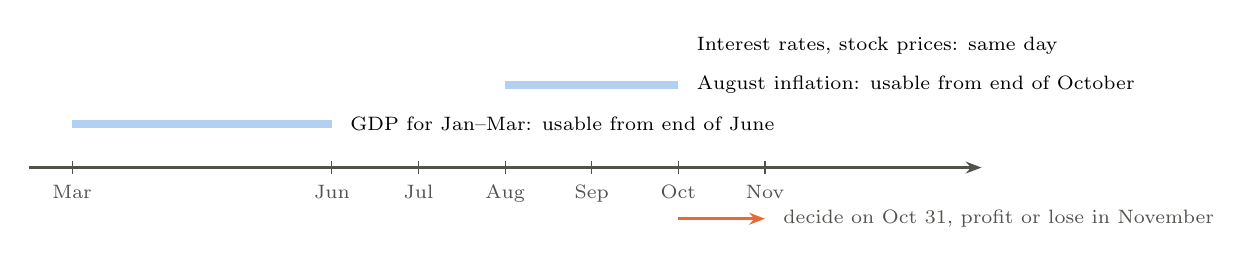
\begin{tikzpicture}[x=1.1cm,y=1cm]
    \draw[line width=0.8pt,color=ink2,-{Stealth[length=2mm]}] (1.5,0) -- (12.5,0);
    \foreach \m/\l in {2/Mar,5/Jun,6/Jul,7/Aug,8/Sep,9/Oct,10/Nov} {
      \draw[color=ink2] (\m,0.08) -- (\m,-0.08);
      \node[below,font=\scriptsize,text=ink2] at (\m,-0.1) {\l};
    }
    \draw[line width=3pt,color=mmblue!35] (2,0.55) -- (5,0.55);
    \node[anchor=west,font=\scriptsize] at (5.1,0.55) {GDP for Jan--Mar: usable from end of June};
    \draw[line width=3pt,color=mmblue!35] (7,1.05) -- (9,1.05);
    \node[anchor=west,font=\scriptsize] at (9.1,1.05) {August inflation: usable from end of October};
    \node[anchor=west,font=\scriptsize] at (9.1,1.55) {Interest rates, stock prices: same day};
    \draw[-{Stealth[length=2mm]},color=tforange,line width=1pt] (9,-0.65) -- (10,-0.65);
    \node[anchor=west,font=\scriptsize,text=ink2] at (10.1,-0.65) {decide on Oct 31, profit or lose in November};
  \end{tikzpicture}
  \vspace{0.6em}

  \small
  \begin{itemize}
    \item Every number is used only after it was published, with a realistic delay.
    \item We check this automatically: scramble all data after some date and confirm nothing before
          that date changes.
  \end{itemize}
  \src{\texttt{signals.PUB\_LAG}; \texttt{tests/test\_pipeline.py}.}
\end{frame}

\begin{frame}{Our data, and how it differs from the paper}
  \footnotesize
  \begin{tabularx}{\textwidth}{@{}l X X@{}}
    \toprule
    & Paper (1970--2016) & Our test (2016--2026) \\
    \midrule
    Economic data & economists' forecasts (paid) & published figures from FRED (free; St.\ Louis Fed) \\
    Interest-rate signal & 2-year bond yield & 3-month rate (stuck near zero 2016--21, so less informative) \\
    Markets & stocks, bonds, currencies, \emph{and} short-term rate futures & stocks, bonds, currencies \\
    Prices & futures contracts & stock indices, bond funds, exchange rates (Yahoo Finance, Fed) \\
    Countries with bonds & 10+ & 6, plus Japan from 2020 \\
    Trading costs & ignored & estimated (next section) \\
    \bottomrule
  \end{tabularx}
  \vspace{0.6em}

  \small Most of these differences make our version weaker than the original, so we expected a lower
  score before running anything. The paper's own last seven years (2010--16) already scored only 0.7.
  \src{\paper; \texttt{README.md}, ``Where this departs from the paper''; \texttt{docs/data.md}.}
\end{frame}

% ===========================================================================
\section{Results}

\begin{frame}{The scorecard}
  \centering\footnotesize
  \resizebox{\textwidth}{!}{\begin{tabular}{l rrrrrr}
\toprule
 & Return per year & Risk (volatility) & Sharpe ratio & $t$-stat & Worst fall & Months up \\
\midrule
Macro momentum & \textbf{7.3\%} & \textbf{10.7\%} & \textbf{0.69} & \textbf{2.2} & \textbf{$-$15.4\%} & \textbf{57\%} \\
Trend following & $-$0.6\% & 10.7\% & $-$0.05 & $-$0.2 & $-$22.8\% & 48\% \\
50/50 & 3.4\% & 8.7\% & 0.39 & 1.2 & $-$9.5\% & 54\% \\
\midrule
Macro momentum, after costs & 6.0\% & 10.7\% & 0.57 & 1.8 & $-$16.5\% & 54\% \\
Trend following, after costs & $-$1.4\% & 10.7\% & $-$0.13 & $-$0.4 & $-$24.0\% & 48\% \\
50/50, after costs & 2.5\% & 8.7\% & 0.29 & 0.9 & $-$9.8\% & 54\% \\
\bottomrule
\end{tabular}
}
  \vspace{0.6em}

  \small
  \begin{itemize}
    \item ``Return per year'' is \emph{above cash}. ``Months up'': share of months with a gain.
    \item The \textbf{$t$-stat} asks ``could this be luck?'' Above about 2 means luck is an unlikely explanation.
          Macro momentum scores \nMMT; trend following is indistinguishable from zero.
  \end{itemize}
  \src{\repo, \texttt{results/summary.md}; \nStart--\nEnd, monthly, every strategy scaled to 10\% volatility.}
\end{frame}

\begin{frame}{What \$100 would have become}
  \centering
  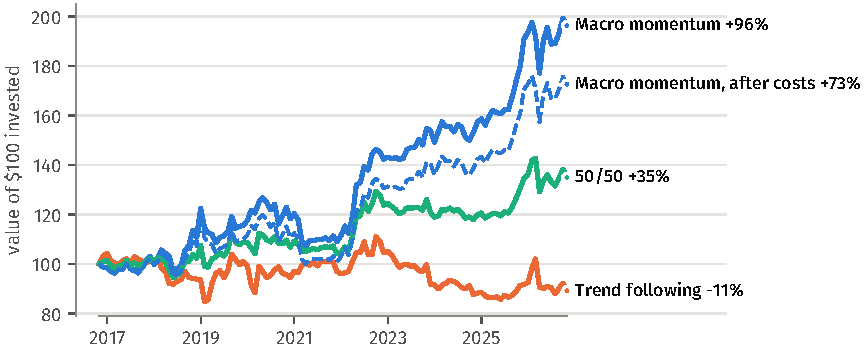
\includegraphics[width=0.84\textwidth]{figs/cumulative.pdf}

  \small Gains \emph{on top of} what cash would have earned. Dashed line: after trading costs.
  Mostly flat until 2022, then big gains in 2022 and 2025.
  \src{\repo, \texttt{results/returns.csv}; \nStart--\nEnd.}
\end{frame}

\begin{frame}{Two very different halves}
  \begin{columns}[c]
    \begin{column}{0.63\textwidth}
      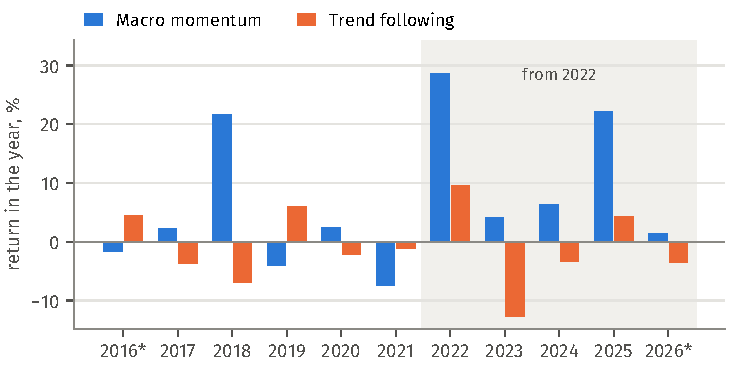
\includegraphics[width=\textwidth]{figs/years.pdf}
    \end{column}
    \begin{column}{0.35\textwidth}
      \small
      Sharpe ratio\\[0.3em]
      \begin{tabular}{@{}lrr@{}}
        \toprule
        & to 2021 & from 2022 \\
        \midrule
        Macro mom. & \nMMFirstHalf & \nMMSecondHalf \\
        Trend & \nTFFirstHalf & \nTFSecondHalf \\
        50/50 mix & \nMixFirstHalf & \nMixSecondHalf \\
        \bottomrule
      \end{tabular}
      \vspace{0.6em}

      Before 2022 interest rates barely moved and countries' economies moved together: little to
      bet on. From 2022 inflation and rates jumped, at different speeds in different countries:
      exactly what the strategy looks for.
    \end{column}
  \end{columns}
  \src{\repo, \texttt{results/calendar\_years.csv}. *2016: Nov--Dec only; 2026: Jan--Oct.}
\end{frame}

\begin{frame}{Which parts worked?}
  \begin{columns}[c]
    \begin{column}{0.57\textwidth}
      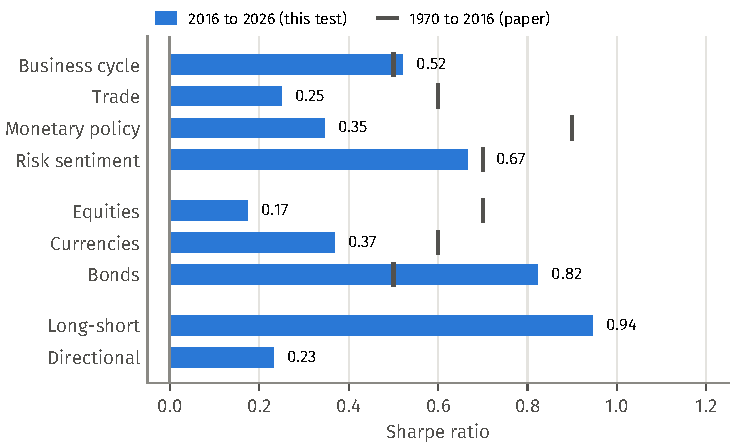
\includegraphics[width=\textwidth]{figs/breakdown.pdf}
    \end{column}
    \begin{column}{0.41\textwidth}
      \small
      Blue bars: our test. Grey ticks: the paper.
      \begin{itemize}
        \item \textbf{Bonds} did even better than in the paper (\nMMBondSharpe).
        \item Among the themes, \textbf{interest rates} fell furthest short of the paper
              (\nMMMonetarySharpe{} vs 0.9), likely because rates sat near zero until 2022.
        \item The \textbf{long-short} version (\nMMXSSharpe) did far better than simple buy/sell (\nMMTSSharpe).
      \end{itemize}
    \end{column}
  \end{columns}
  \src{\repo, \texttt{results/stats.csv}; paper figures from \texttt{docs/paper\_summary.md}. Paper has no long-short/simple split.}
\end{frame}

\begin{frame}{Trading isn't free}
  \begin{columns}[c]
    \begin{column}{0.52\textwidth}
      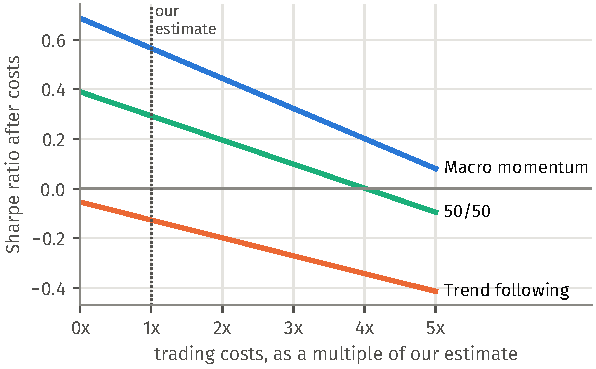
\includegraphics[width=\textwidth]{figs/costs.pdf}
    \end{column}
    \begin{column}{0.46\textwidth}
      \small
      \begin{itemize}
        \item Every trade pays a small fee (the gap between buying and selling prices).
        \item The strategy trades a lot: about \textbf{\nMMTurn{} times its own value per year}, mostly in bonds.
        \item Our estimate: 0.03--0.04\% per trade. That costs about \nMMDrag{} a year and lowers the Sharpe
              from \nMMSharpe{} to \nMMNetSharpe.
        \item We don't know the true cost, so the chart shows what happens if it is 2, 3, 4 or 5 times higher.
              At 4 times our estimate, little is left (\nMMSharpeFour).
      \end{itemize}
    \end{column}
  \end{columns}
  \src{\repo, \texttt{results/costs.csv}; cost estimate (\nCostEq, \nCostBond, \nCostFx\ basis points for stocks, bonds, currencies) in \texttt{mm.backtest.COST\_BPS}.}
\end{frame}

\begin{frame}{Speed matters}
  \centering\small
  \begin{tabular}{l rrr rr}
\toprule
Trade & \multicolumn{3}{c}{Sharpe ratio, before costs} & \multicolumn{2}{c}{after costs} \\
\cmidrule(lr){2-4}\cmidrule(lr){5-6}
 & Macro mom. & Trend & 50/50 & Macro mom. & Trend \\
\midrule
right away & 0.69 & $-$0.05 & 0.39 & 0.57 & $-$0.13 \\
one month late & 0.65 & $-$0.20 & 0.27 & 0.52 & $-$0.28 \\
two months late & 0.21 & $-$0.02 & 0.11 & 0.09 & $-$0.09 \\
\bottomrule
\end{tabular}

  \vspace{0.8em}

  \begin{itemize}
    \item What if you act on the signal one or two months later than you could have?
    \item One month late: almost no harm. Two months late: most of the edge is gone.
    \item Small choices like this move a ten-year result a lot, one more reason to be cautious.
  \end{itemize}
  \src{\repo, \texttt{results/sensitivity.csv}; same ten-year window in every row.}
\end{frame}

% ===========================================================================
\section{Versus trend following}

\begin{frame}{Do the two strategies move together?}
  \begin{columns}[c]
    \begin{column}{0.62\textwidth}
      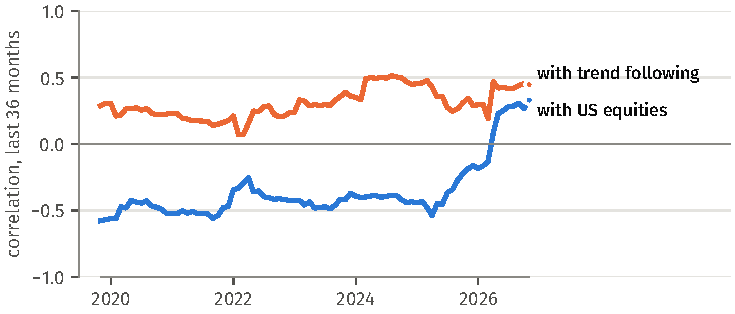
\includegraphics[width=\textwidth]{figs/rollcorr.pdf}
    \end{column}
    \begin{column}{0.36\textwidth}
      \small
      \textbf{Correlation}: $+1$ = always move together, 0 = unrelated, $-1$ = always opposite.
      Low correlation is good: one can make money when the other loses.
      \vspace{0.4em}

      Over the whole decade, macro momentum's correlation was \nCorrMMTF{} with trend following and
      \nCorrMMEq{} with US stocks (paper: 0.4 and $-$0.22).
      In 2026 the link with stocks turned positive.
    \end{column}
  \end{columns}
  \src{\repo, \texttt{results/correlations.csv}; rolling 36 months. Paper: \texttt{docs/paper\_summary.md}.}
\end{frame}

\begin{frame}{Trend following had a bad decade here}
  \begin{itemize}
    \item On the same 26 markets: Sharpe \nTFSharpe{} before costs, \nTFNetSharpe{} after, against 1.1 in the paper.
    \item Its worst years were 2023 and 2018. 2022, the year of big moves, was its best.
    \item The \textbf{50/50 mix}, half in each strategy (Sharpe \nMixSharpe), did \emph{worse} than macro momentum alone,
          because trend following added ups and downs but no profit. In the paper the mix was the best of the three.
    \item Lesson: combining strategies only helps if each one earns something on its own.
  \end{itemize}
  \vspace{0.3em}
  \small Not a final verdict on trend following: this is one decade, few markets, and a simple version.
  \src{\repo, \texttt{results/summary.md}, \texttt{results/calendar\_years.csv}; \paper.}
\end{frame}

% ===========================================================================
\section{Wrap-up}

\begin{frame}{What to take away, and what we can't say yet}
  \begin{columns}[T]
    \begin{column}{0.48\textwidth}
      \textbf{Takeaways}
      \small
      \begin{itemize}
        \item The idea survived ten new years, at about half the original strength.
        \item It paid off mostly when economies diverged (2022 onwards).
        \item Trading costs and timing matter a lot.
      \end{itemize}
    \end{column}
    \begin{column}{0.5\textwidth}
      \textbf{Limits}
      \small
      \begin{itemize}
        \item Ten years is short: the Sharpe could easily be $\pm$\nSharpeSE{} off.
        \item Economic figures get revised later; we use today's version, not what people saw then.
        \item Free inflation data stops early for 5 of 10 countries.
        \item Trading costs are our estimate, not measured.
        \item A backtest is a simulation. Not investment advice.
      \end{itemize}
    \end{column}
  \end{columns}
  \src{\repo, \texttt{README.md} (Known gaps), \texttt{results/data\_qa.md}.}
\end{frame}

\begin{frame}{Glossary}
  \footnotesize
  \begin{columns}[T]
    \begin{column}{0.49\textwidth}
      \begin{description}[Out of sample]
        \item[Backtest] simulating a rule on past data.
        \item[Basis point] 0.01\%. 4 basis points = 0.04\%.
        \item[Bond] a loan to a government that pays interest; price falls when rates rise.
        \item[Correlation] how closely two returns move together, from $-1$ to $+1$.
        \item[CPI, inflation] consumer price index; inflation is its change over a year.
        \item[Drawdown] fall from a previous high.
        \item[GDP] total output of an economy.
        \item[Long / short] betting on a rise / a fall.
      \end{description}
    \end{column}
    \begin{column}{0.49\textwidth}
      \begin{description}[Out of sample]
        \item[Macro] the economy as a whole.
        \item[Momentum] the tendency of a trend to continue for a while.
        \item[Out of sample] tested on data the rules were not built on.
        \item[Return above cash] gain minus what a bank deposit would have paid.
        \item[Sharpe ratio] return divided by volatility.
        \item[$t$-stat] how unlikely a result is to be luck; above 2 is the usual bar.
        \item[Trend following] buying what has risen, selling what has fallen.
        \item[Volatility] how much returns swing; our measure of risk.
      \end{description}
    \end{column}
  \end{columns}
\end{frame}

\begin{frame}{Sources}
  \small
  \begin{itemize}
    \item Brooks, J. (2017). \emph{A Half Century of Macro Momentum}. AQR Capital Management.
          \url{https://www.aqr.com/-/media/AQR/Documents/Insights/White-Papers/A-Half-Century-of-Macro-Momentum.pdf}
    \item Federal Reserve Bank of St.\ Louis, FRED (\url{https://fred.stlouisfed.org}): GDP, CPI, interest rates,
          BIS trade-weighted exchange rates, Fed H.10 exchange rates. Series ids in \texttt{src/mm/universe.py}.
    \item Yahoo Finance: stock indices and government bond funds, month-end prices.
          Tickers in \texttt{src/mm/instruments.py}.
    \item Code, data and every number in this deck: \url{https://github.com/chkoh89/macro-momentum}.
          Figures and numbers are generated by \texttt{scripts/make\_deck\_assets.py}.
  \end{itemize}
\end{frame}

\end{document}
